\documentclass{altsu-bachelor}
\linespread{1,5}

\begin{document}

\begin{titlepage}
 \begin{center}
    \normalsize
    МИНИСТЕРСТВО НАУКИ И ВЫСШЕГО ОБРАЗОВАНИЯ \\
    РОССИЙСКОЙ ФЕДЕРАЦИИ \\
    ФГБОУ ВО «АЛТАЙСКИЙ ГОСУДАРСТВЕННЫЙ УНИВЕРСИТЕТ»
    \vfill
     
    Институт цифровых технологий, электроники и физики (ИЦТЭФ) \\
    Кафедра вычислительной техники и электроники (ВТиЭ)
    \vfill
     
    \textbf{Разработка и отладка параллельной MPI-программы для метода Якоби сеточного решения уравнения Лапласа}
    
    Отчет по лабораторной работе №2
 \end{center}
\vfill
 
\newlength{\ML}
\settowidth{\ML}{«\underline{\hspace{3cm}}»}
\hfill\begin{minipage}{0.41\textwidth}
  Выполнил: студент гр. 5.306M\\
  \underline{\hspace{\ML}} А.\,В.~Лаптев \\
  Проверил: ст. преп. кафедры ВТиЭ\\
  \underline{\hspace{\ML}} И.\,А.~Шмаков \\
  «\underline{\hspace{1cm}}» \underline{\hspace{3cm}} \the\year г.
\end{minipage}%
\vfill
 
\begin{center}
  Барнаул, \the\year г.
\end{center}
\end{titlepage}

\setcounter{page}{2}
\tableofcontents
\newpage

\section*{Цель работы}
\addcontentsline{toc}{section}{Цель работы}

Изучить метод Якоби, проанализировать приведенный текст параллельной программы этого метода, который необходимо дополнить недостающими блоками для того, чтобы программа отрабатывала без ошибок и корректно решала поставленную задачу.

\section*{Задание}
\addcontentsline{toc}{section}{Задание}

\begin{enumerate}
    \item изучить метод Якоби, изложенный в Приложении (имя файла <<Метод\_итераций\_Якоби.doc>>). Проанализировать ниже приведенный текст параллельной программы этого метода, который необходимо дополнить недостающими блоками для того, чтобы программа отрабатывала без ошибок и корректно решала поставленную задачу;
    
    \item после доработки и успешной отладки программы определяются Граничные условия на искомую функцию поверхности (решения уравнения Лапласа), заданные на сторонах прямоугольной сеточной области. Образец задания показан ниже в примере выполнения программы.
\end{enumerate}

\section*{Выполнение работы}
\addcontentsline{toc}{section}{Выполнение работы}

После изучения метода Якоби был рассмотрен текст программы, в который были внесены некоторые изменения и дополнения. Далее будут описаны те изменения, которые были внесены.

\subsection*{Изменения исходного кода}
\addcontentsline{toc}{subsection}{Изменения исходного кода}

Первым шагом было добавлено считывание размера сетки и количества итераций для обмена границ внутри сетки, а также добавлен расчет размера полосы, который будет обрабатываться одним потоком/процессором.

Следующим шагом был добавлен вывод результатов для рассчитанной погрешности в переменную \textit{maxdiff}.

После чего были инициализированы матрицы, содержащие граничные условия, матрицы были инициализированы нулями. Также было добавлено определение соседей справа и слева от текущего значения внутренней сетки (исключая границы).

В самом конце была вычислена собственная погрешность расчетов \textit{mydiff}, которая вычисляется как максимальное значение между текущим ее значением и модулем разности между новым и старым значением конкретной ячейки в сетке.

\subsection*{Обработка результатов работы программы}
\addcontentsline{toc}{subsection}{Обработка результатов работы программы}

В результате работы программы был сформирован текстовый файл со всеми необходимыми исходными данными для построения графика.

Ниже будет представлено несколько графиков, которые отображают зависимость различных параметров, используемых в расчетах друг от друга.

На данном графике приведено <<седло>>, которое получается при тестовых Граничных Условиях, до получения персональных, а именно функция решения уравнения Лапласа удовлетворяет Граничным Условиям $\Phi = 1 = const$ вдоль одной размерности и условию $\Phi = 0 = const$ вдоль другой размерности.

\begin{figure}[H]
    \centering
    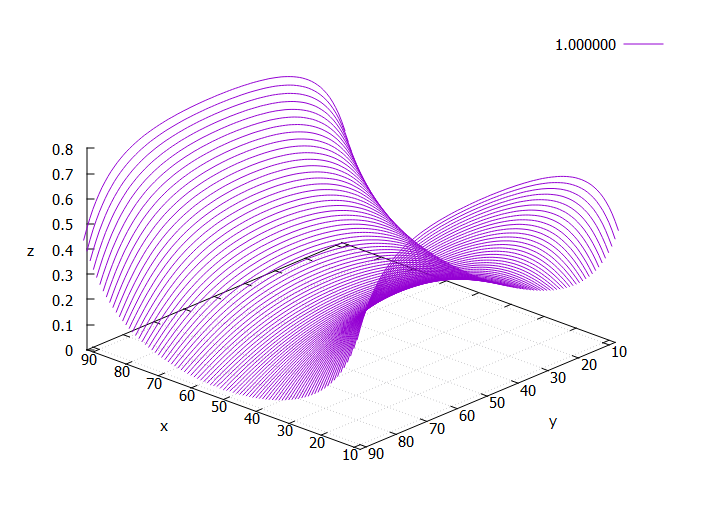
\includegraphics[scale=0.65]{saddle.png}
    \caption{\centering Трехмерное изображение поверхности , удовлетворяющее уравнению Лапласа и Граничным Условиям.}
    \label{fig:saddle}
\end{figure}

Ниже представлен график для персональных Граничных Условий, а именно: $\Phi_L = const = 12$, $\Phi_U = const = 11$, $\Phi_R = const = 4$, $\Phi_D = const = -1$. 

\begin{figure}[H]
    \centering
    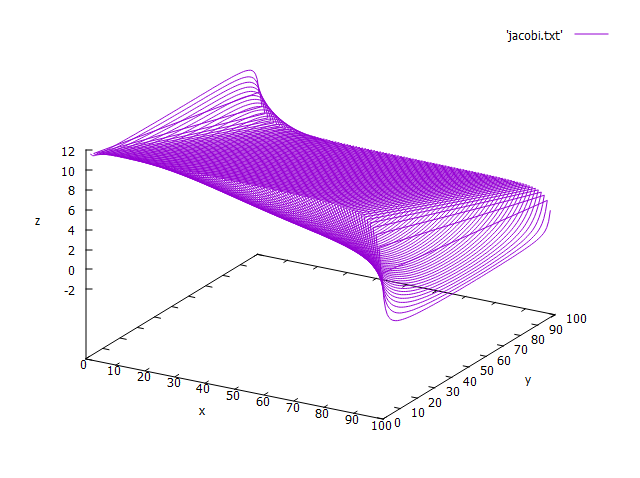
\includegraphics[scale=0.65]{personal_figure.png}
    \caption{\centering Трехмерное изображение поверхности, удовлетворяющее уравнению Лапласа и персональным Граничным Условиям.}
    \label{fig:myfigure}
\end{figure}

\section*{Вывод}
\addcontentsline{toc}{section}{Вывод}

В ходе выполнения работы было осуществлено знакомство с методом Якоби для решения сеточного уравнения Лапласа и изучена его программная реализация. Были внесены необходимые изменения и дополнения в код и построены графики с различными Граничными Условиями.

\newpage
\chapter*{\begin{flushright}Приложение\end{flushright}}
\addcontentsline{toc}{chapter}{Приложение}

\begin{code}
\captionof{listing}{\label{code:jakobi}Исходный код для расчета методом Якоби}
\vspace{0.5cm}
{\small
\inputminted[mathescape,linenos,frame=lines,breaklines]{C++}{jakobi.c}
}
\end{code}

\end{document}
